\documentclass[11pt]{article}

\usepackage[top=0.5in, bottom=0.5in, left=0.5in, right=0.5in]{geometry} 
\usepackage{graphicx}
\usepackage{url}
\usepackage{indentfirst}

\begin{document}

\vspace{5cm}
\title{Box2D Simulation of a Radial Engine}
\author{Pratik Fegade 120050004\\M. S. Krishna Deepak 120050057\\P. Bharath Kumar 120050058\\}
\maketitle
\pagebreak
\tableofcontents
\pagebreak
\section{Introduction}
A radial engine is an engine that has a certain number of cylinders arranged circularly to rotate a central shaft. This shaft can be then used to drive a propeller of an aircraft. An image\cite{radEng} of a radial engine is given below.

\begin{center}
	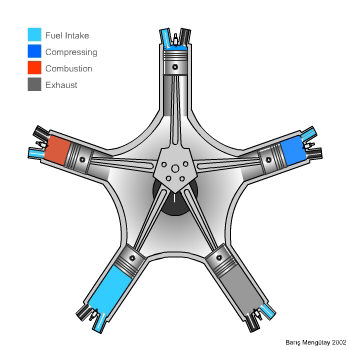
\includegraphics[width=12cm]{./images/radEng.jpeg}
\end{center}

\subsection{Our Project}
This simulation was done as a project for the course Software Systems Lab (CS296). This report describes the simulation as was originally proposed at the start of the semester and as it finally turned out. Also, it includes the analysis of the profiling data obtained by profiling the simulation (without the GUI and the graphics). Some drawbacks of the simulations are also discussed.

\pagebreak

\section{Initial Proposal}
The initial proposal is summarised in the image below.
\begin{center}
	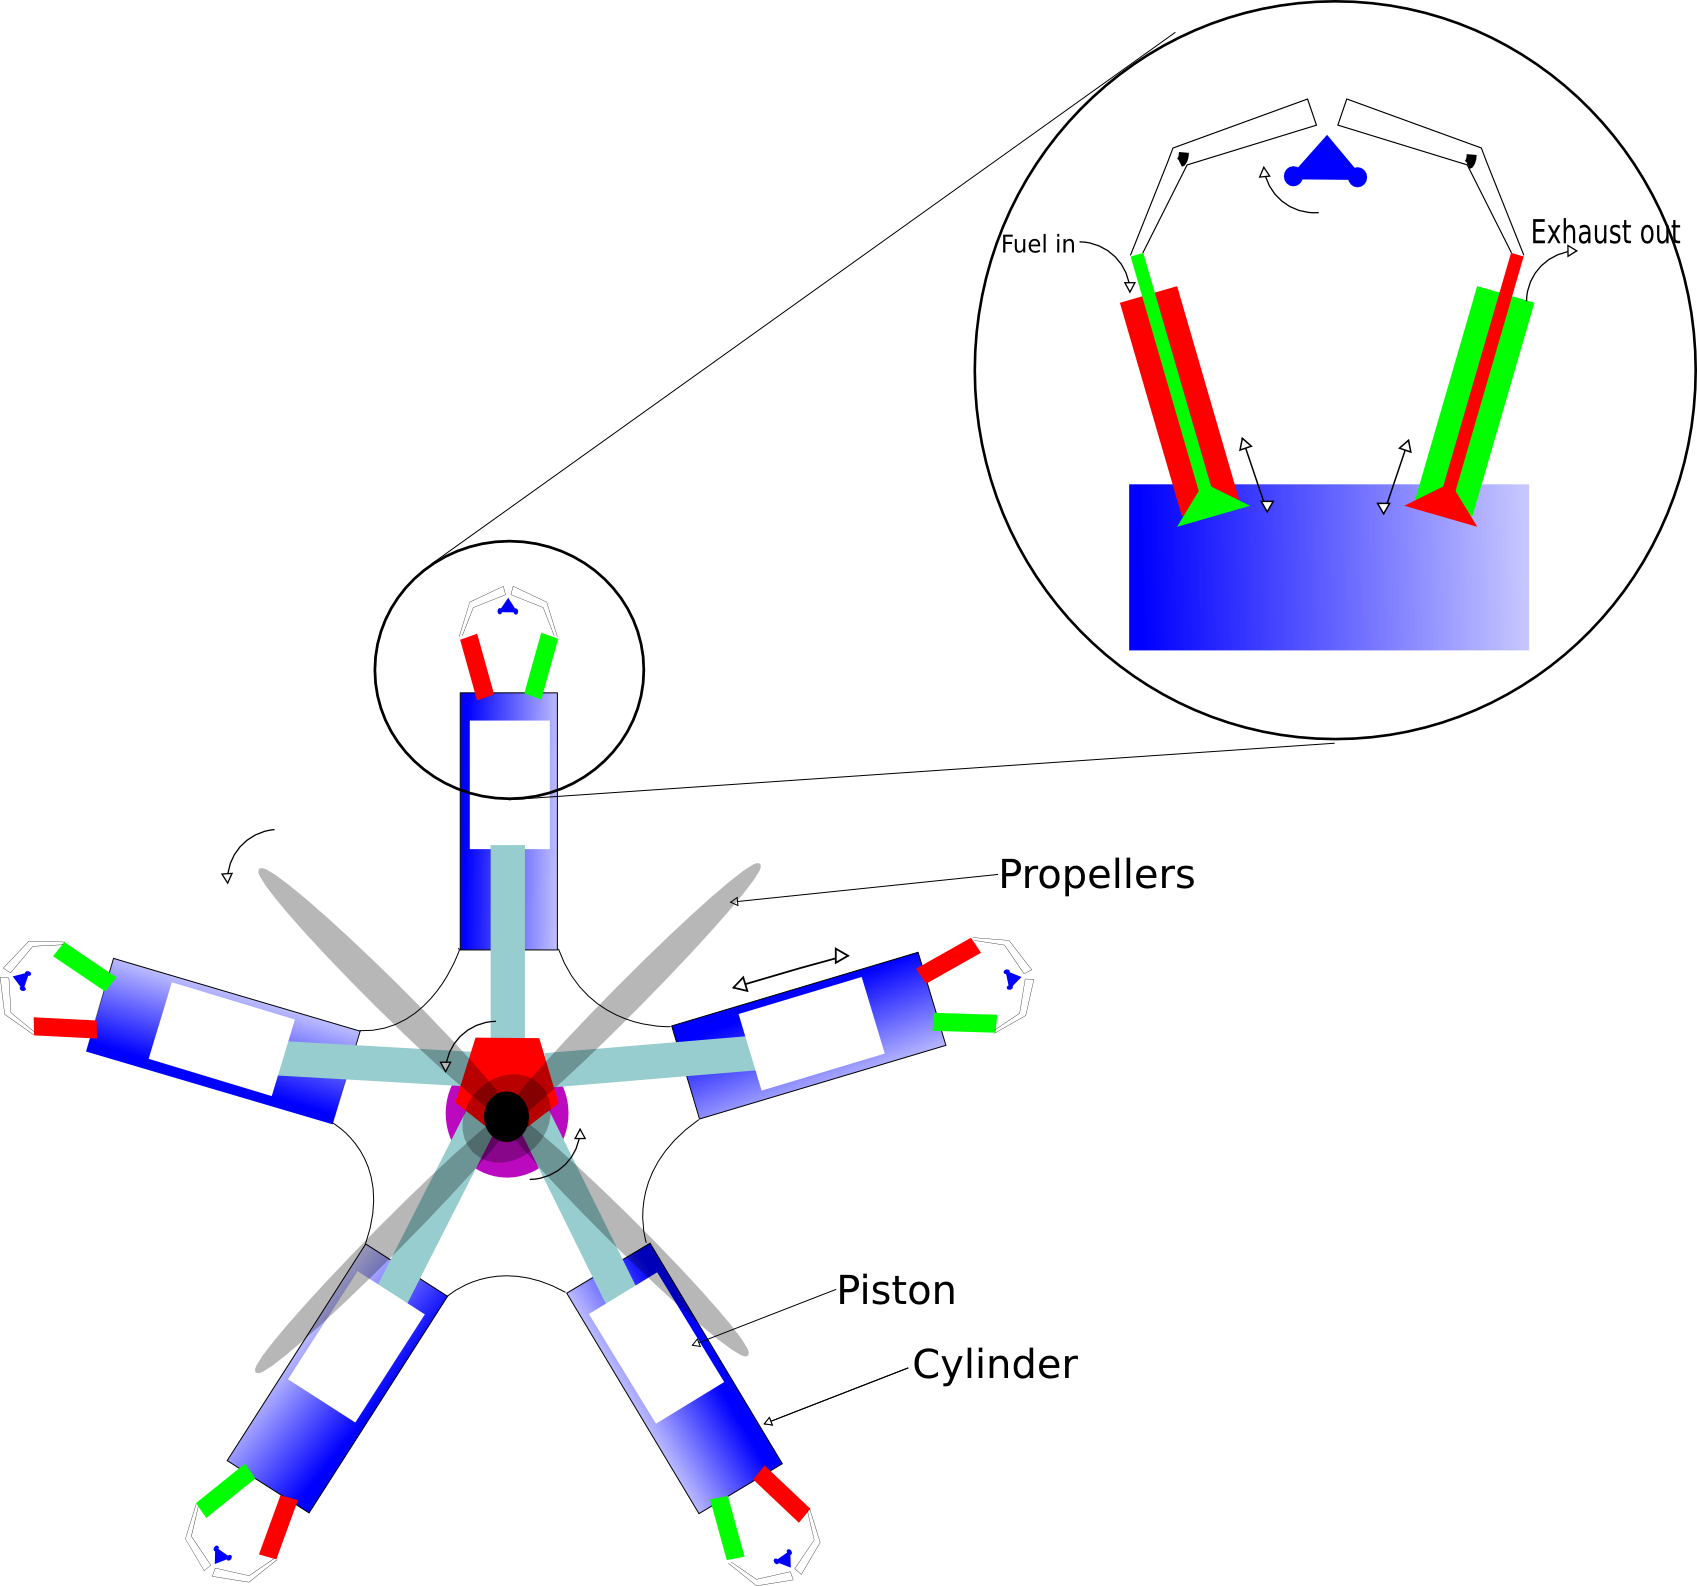
\includegraphics[width=12cm]{./images/initialProposal.png}
\end{center}
\pagebreak
\section{The Final Simulation}
A screenshot of the final simulation is given below
\begin{center}
	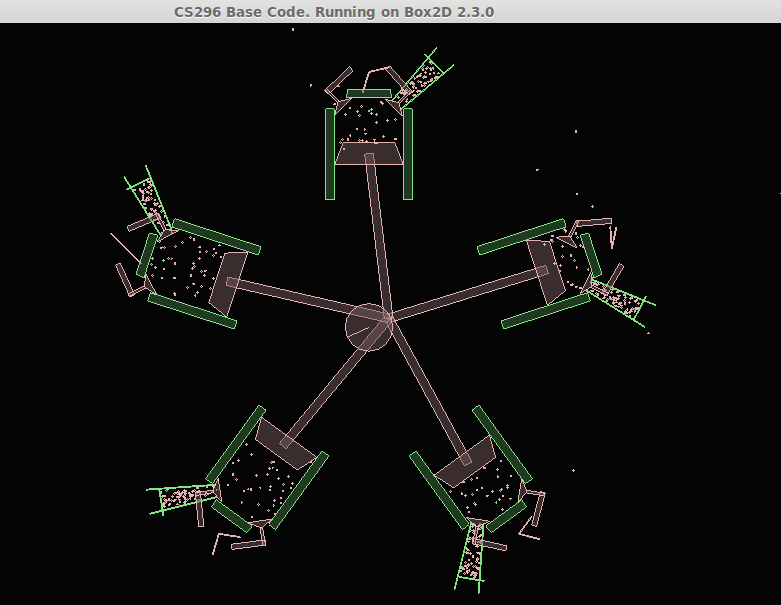
\includegraphics[width=12cm]{./images/fullReport.png}
\end{center}

\indent As can be seen, there are not any significant differences between the proposed simulation and the final submission although the dimensions are not in general the same in the proposed and the final simulation.
\indent Some additional screenshots of the simulation are given below.

\begin{center}
	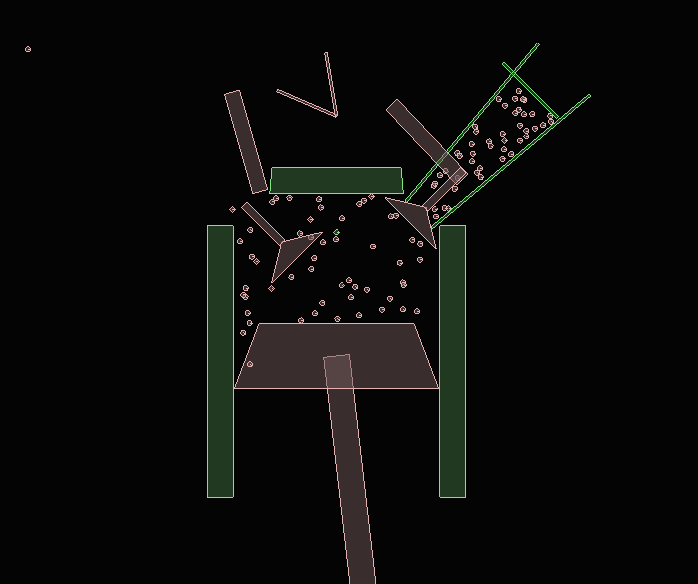
\includegraphics[width=12cm]{./images/exhaustOpenReport.png}
\end{center}

\section{Some Interesting Points}

\subsection{Synchronisation}
As mentioned earlier(in Drawbacks/Limitations of the Simulation), one could observe that the fuel intake and exhaust are synchronised at the start as in a 4-Stroke Engine. This was made by setting the angular velocities of Planks at exhaust and at fuel 1/2 of the angular velocity of `piston Sphere'(The Circle shaped thing situated at (0,0)) and also setting the initial angles of planks in 5 cylinders appropriately.
\begin{center}
\begin{verbatim}
		if (fuelPlankJoint[i] != NULL){
			fuelPlankJoint[i]->SetMotorSpeed(0.5f * pistonSphere->GetAngularVelocity());
		}
		if (exhaustPlankJoint[i] != NULL){
			exhaustPlankJoint[i]->SetMotorSpeed(0.5f * pistonSphere->GetAngularVelocity());
		}


\end{verbatim}
\end{center}

\subsection{Others}
We have used formulae for transformation and rotation of axes to generate 5 similar cylinders around the `piston Sphere' and hence have effectively written code for only one cylinder and repeated this code 5 times with different parameters.

We have overridden the step function of base\_sim\_t class in dominos\_t class and have used it to check for specific things in each step of simulation.

We have also used the EndContact method in b2ContactListener class to change some parameters(like userdata) of specific bodies when they collide.

\section{Analysis of the plots}
The data is obtained by running the simulation for some reruns for a particular number of steps and averaging over the reruns. Data for loop time, step time, time required for position, collision and velocity updates was collected. The step time is significantly high for low number of iterations (probably due to all the variable initialisations required at the start of the simulation) and it falls quickly and stabilises. Similar but less pronounced effects are seem with the times required for velocity, position and collision updates. Also the sum of the average times required for velocity, position and collision updates significantly falls short of the average step time suggesting that some other not examined function takes up significant amounts of time. For all the iteration values, the velocity update time is the highest while the collision update time is the lowest. The plot is shown below.

\begin{center}
	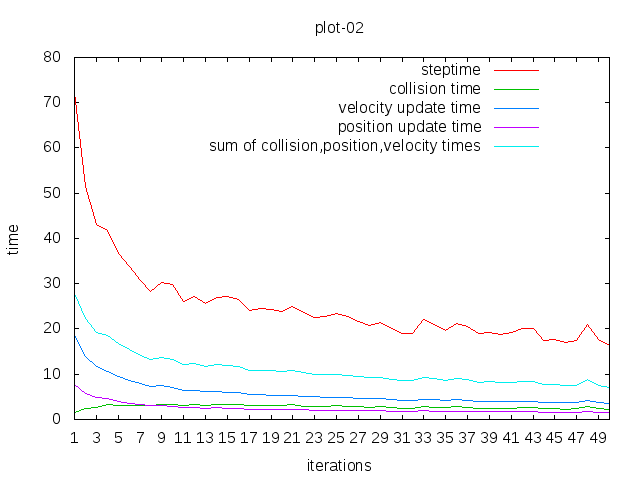
\includegraphics[width=12cm]{./images/plots/g04_plot02.png}
\end{center}

\indent The collision time, as is seen in the plot above, initially is low and then is rises to a higher value. This is probably due to the fact that at the start of the simulation, the gas particles (which contribute to most of the collisions) are not colliding with the cylinder walls or/and the piston as they are all in the fuel intake region of the engine.
\\
\indent The simulation contains 592 bodies, 60 joints and around 4000 contacts are present at any time in the simulation (this information is obtained from Box2D statistics as are displayed in the GUI). The original base code had 34 bodies, 4 joints and around 40 contacts at any time in the simulation. The average step time for the project came out to be around 25 ms. Also the average step time for the original bas code was computed to be around 0.3 ms. That is an increase by a factor of about 80. The bodies however have not increased in this proportion, the contacts have increased by a factor of about 100. Thus the total time required to compute the contacts and hence the collisions scales as per the number of the contacts. This is not however true for the number of bodies or the number of the joints.


\indent The average step time for a significant number of iterations is almost stable though it sometimes varies a lot over the reruns. This is demonstrated by plotting a frequency plot of the step times over the reruns for a particular value of the number of iterations. The plot as expected shows a concentrations of step times around the average step time but it does have a significant tail as a result of some high values of the step time. A plot demonstrating this is shown below.

\begin{center}
	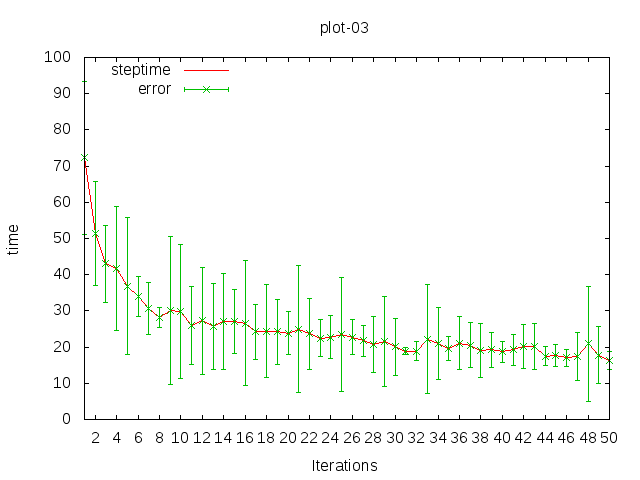
\includegraphics[width=12cm]{./images/plots/g04_plot03.png}
\end{center}

\indent The data was generated for 20 reruns for each iteration (1 to 50). However, a plot of the line obtained by applying linear regression on  average step time of randomly selected 10 reruns out of the 20 reruns shows striking similarity to that obtained by regressing over the entire data. Hence it seems that the analysis would not differ much even if data is collected for a smaller number of reruns. A plot demonstrating this is shown below.

\begin{center}
	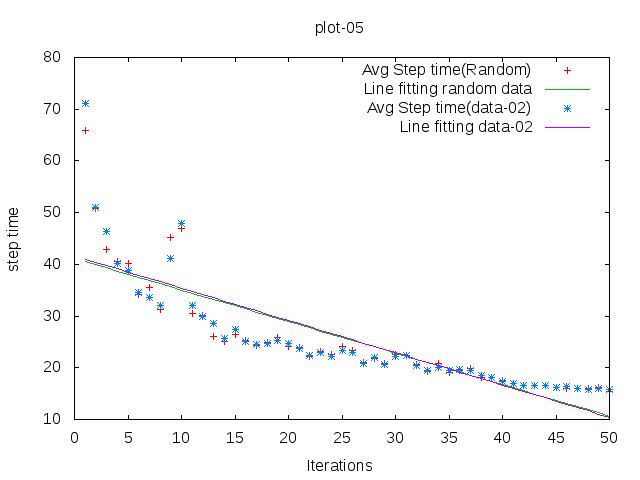
\includegraphics[width=12cm]{./images/plots/g04_plot05.png}
\end{center}

\section{Analysis of the Profiling Data}
The profiling data for the simulation was generated by running it for 50,000. Most of the functions in the simulation source code should have been called and hence profiled as the simulation was run for 50,000 steps. The profiler perf\cite{perfsite} was used to generate the data. Following is analysis of the data of both the release and the debug builds of the simulation and a comparison of both.

\subsection{Analysis of the Release Build}
 In the case of the release build, the b2World::SolveTOI(b2TimeStep const\&) function takes the maximum amount of time (about 8.52\% of the total) amongst all the functions profiled. This is followed by the void b2DynamicTree::Query<b2BroadPhase>(b2BroadPhase*, b2AABB const\&) function and the b2Island::Solve(b2Profile*, b2TimeStep const\&, b2Vec2 const\&, bool) function. The b2World::SolveTOI(b2TimeStep const\&) function is used to predict the time of collision of two bodies so as to avoid tunnelling\cite{solveTOI}. This takes a significant amount of time as there are a lot of bodies (the gas particles) in the simulation. Libraries that are not a part of the Box2D package and that take a significant amount of time are as follows

\begin{itemize}
\item vdso (virtual ELF dynamic shared object)\cite{vdso} : This shared object is called by the C library. It takes about 20\% of the total time.
\item libm-2.17.so : It takes about 8\% of the total time
\end{itemize}

\subsection{Analysis of the Debug Build}
Excluding the functions related to GLUI or GLUT and overloaded operators performing subtraction and multiplication of b2Vec2 objects, b2World::SolveTOI(b2TimeStep const\&) took the most percentage of time (about 1.90\%). Operators in totality take about 10\% of the total time. Also, an interesting point to note is that the b2Vec2::b2Vec2(float, float) constructor takes 3.53\% of the total time. this explains why the operators are called for such a large number of times. There are too many b2Vec2 objects being constructed and performed computations upon. The b2World::SolveTOI(b2TimeStep const\&) function might need to create these objects for its computations. The shared libraries vdso and libc-2.17.so (The C library most probably) also consume a lot of time.

\indent Another class functions that we found interesting were the methods of the class b2DynamicTree. This class is used for data organisation by box2D (i.e. to store the list of AABBs of the bodies)\cite{dynamicTree}. These functions are used a lot in the simulation as there are a number of bodies in the simulation. 
\\
\indent We thus observe that most of the functions that feature in the profiling data relate to physical computations for the bodies. Thus reducing the number of bodies(mainly the number of the gas particles) would help quicken the simulation. This may be done by increasing the density/velocity of the particles and reducing the number. However, increasing the velocities leads to the particles jumping boundaries as explained in section 6.1.
\section{The Call Graph}
The call graph generated for the debug build by perf is shown on the previous page. As the call graph shows, the execution of the C++ code starts with the execution of \_\_libc\_start\_main in the library libc-2.17.so which later calls the main function of the simulation. Also, it is seen that most of the functions execute within a reasonable amount of time and that only some functions take an extraordinarily large amount of time.

\begin{center}
	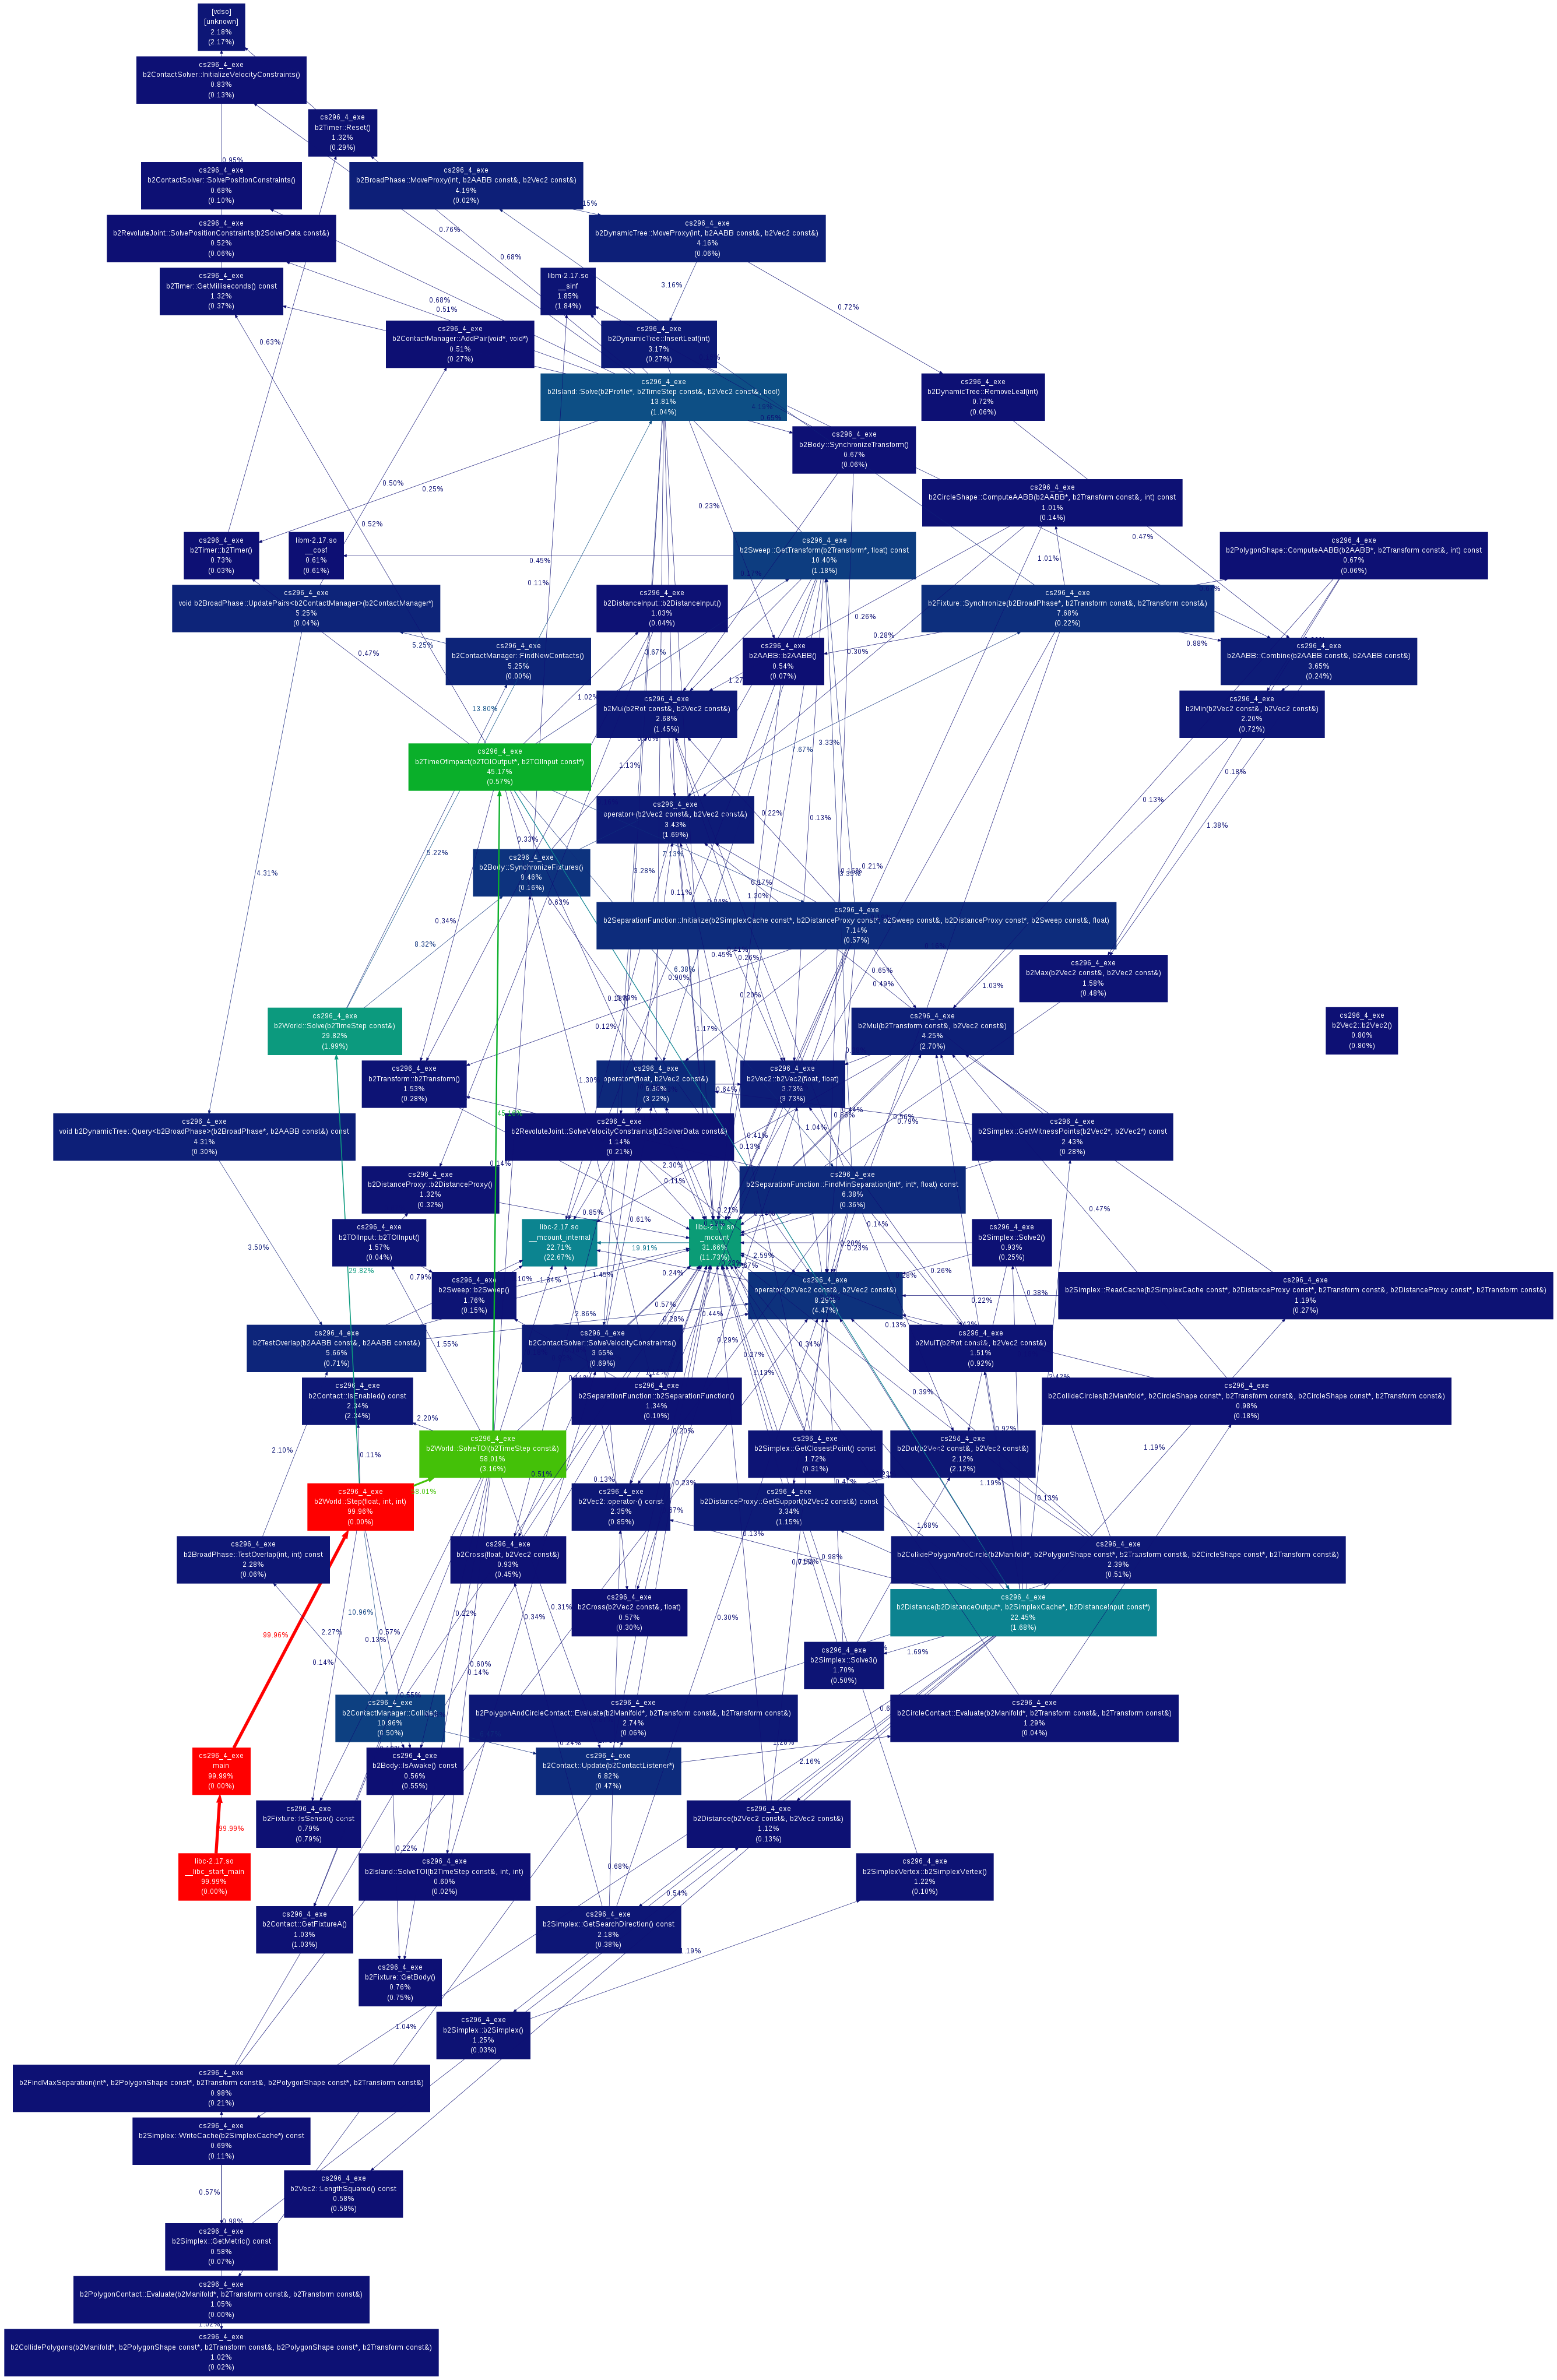
\includegraphics[height=25cm]{./images/plots/fdp.png}
\end{center}

\section{Drawbacks/Limitations of the Simulation} 
The following are the drawbacks in the simulation we have identified
\subsection{Escaping Gas Particles}
Due to their high velocities, the gas particles advance a significant distance in one step of the simulation. As a result they frequently escape through the body walls in the simulation. In order to counter, we have destroyed particle that escape the cylinder and re-spawned them back in the fuel intake region. This may be solved by increasing the mass of the particles and reducing their velocities.
\subsection{Fuel Intake and Exhaust not Synchronised}
We have not been able to properly synchronise the timings of the piston and the fuel intake and the exhaust. The synchronisation is satisfactory at the start of the simulation however it degrades as the simulation progresses.
\subsection{Slow Engine}
The rpm of the engine is particularly slow. This might be due to the low momentum transfers from the gas particles to the piston or due to the lack of proper synchronisation as described above.
\subsection{No Sparking}
We have not implemented a special sparking event in the engine. Instead there is always an `ignited'  particle in the cylinder and if an `un-ignited' particle comes in contact with it, it is ignited (gains mass).
% \begin{itemize}
% \item Find plans.
% \item Save world.
% \item Get out of my house!
% \end{itemize}

% \indent In both the above cases, as the number of iterations the simulation is run for rises, the time taken by b2ContactSolver::SolveVelocityConstraints() relative to the total time remains almost constant. Similar is the case with the other functions that take significant amount of time. For a smaller number of iterations some functions in  libraries like [kernel.kallsyms] take a large portion of the total running time. However this is not observed with large number of iterations probably because they take a constant amount of time to execute independent of the number of the iterations.
% \subsection{A Comparison of Debug and Release Data}
% The profile generated for the debug build is significantly larger than the one for the release build (compiled with level 3 optimisation). This makes the debug profile much more informative and fine-grained and hence easier for debugging the code. The debug profile most significantly contains the overhead data for all the operators defined for the various structs (vectors and similar objects) used in the simulation. Also, it includes the data for the constructors and destructors of the classes. It turns out that these do consume a significant amount of the total time. This critical information is not however, accounted for in the release version profile.
% \\
% \indent The -03 or -o2 options given to g++ during compilation tell the compiler to optimise the code to a desired level (2 or 3 in this case). The profiler can generate so much more information in the case of the debug build as the compiler consider statements as independent and hence does not optimise the code when complied in the debug mode. As a result the functions which the compiler would normally optimise (like constructors, destructors and operators) are left as they are and hence the compiler can then insert appropriate debug symbols for each of these functions (and hence the debug build is significantly larger than the release build) thus enabling the profiler to gather data about these functions. In the release build the compiler highly optimises the code and all the functions it optimises are unobservable as far as the profiler is concerned.
% \\
% \indent As the both the release and the debug profiles suggest, the b2ContactSolver::SolveVelocityConstraints() function is the one that if improved/optimised would lead to faster simulations. Also, as is evident from the debug profile, the operators - especially operator\*(float, b2Vec2 const\&) and operator\-(b2Vec2 const\&, b2Vec2 const\&) are used often and hence an improvement in their implementations would affect the performance of the simulation. Also, one might try to reduce the number of calls to these operators/functions by some means.
% \\


\bibliographystyle{plain}
\bibliography{cs296_g04_project_report.bib}

\end{document}
